\chapter{Constructing a Cardiac Simulation Toolkit}
\label{chapter:toolkit}

The cardiac simulation toolkit was developed to provide a more systematic
framework for exploring the properties of cardiac cell and tissue models.
It does this through offering a uniform and simple cell interface, a series of
standardised pacing protocols and facilities for two dimensional simulations.
It is intended to be easy to script to make constructing more complex numerical
experiments as easy as possible.

Existing cardiac simulation toolkits offer graphical interfaces and require
specification of the desired protocol through such interfaces.
The toolkit instead has inbuilt knowledge of several simulation protocols.
This ensures different investigations use the same protocols, allowing results
to be compared more directly.
In addition, by performing specific simulation protocols with a dedicated
program, performance optimisations specific to a given protocol are possible.

The toolkit proposed in this chapter allows many aspects of the simulation,
including the parameters used in the model, to be specified on the commandline
or via simple configuration files.
By allowing such control potentially boring and time consuming investigations,
such as investigating how a property varies with the alteration of a parameter
or set of parameters, can be driven externally rather than via repeated manual
alterations.
This both reduces errors and increases productivity.

The toolkit therefore offers an extensible environment for performing cardiac
simulations.
It has inbuilt knowledge of several experimental protocols.
No existing simulation toolkit offers these features.


\section{Simulation Environment}

The simulation environment provided by the cardiac toolkit is intended to be as
portable as possible, so that numerical experiments may be run on whichever
platforms are appropriate.  To this end, all the data input structures are based
on open standards, or simple binary formats.  The output formats provided by the
various driver programs are also in simple binary or ASCII formats, to allow
them to be easily visualized with both commercial and open source visualisation
tools.  The results presented later in this chapter were performed on desktop
computers with a Athlon X2 3600+ chip and 1 GB RAM and on Horace, the local HPC
facility.  Horace has 24 compute nodes, each one consisting of four Intel Itanium2
Montecito Dual Core 1.6GHz processors, 16GB RAM and up to 512GB of local scratch
space.  The nodes are connected by a high speed Quadrics QsNetII
interconnect.  Horace provides compilers for both Fortran and C,
and for both the MPI and OpenMP parallelization libraries.

\subsection{Implementation}

The experimental protocol drivers and the cellular models were implemented in
the C programming language.
Much of the supporting code and supplementary tools were implemented in the ruby
programming language~\cite{Flanagan2008}.
The cellular models currently implemented are based on the Hodgkin-Huxley
formalism, although there is no fundamental reason why a Markov chain based
model could not be included.
Inter-cellular coupling for propagation of excitation over a strand or tissue
was implemented using the monodomain equations.

\subsubsection{Cellular Models}

The cellular model used for much of the developmental process was the
Courtemanche et al. human atrial myocyte model~\cite{CRN98}.
Also currently implemented is the four variable formulation of the Fenton-Karma
minimal variable model~\cite{Bueno-Orovio2008}.
These cellular models describe the behaviour of a cell using coupled systems of
non-linear ordinary differential equations.
The ODEs represent the concentrations of intra- and extra-cellular ion species
and the flow of current through ionic channels in the cell membrane or between
intra-cellular compartments, or their notional equivalents in the case of
minimal variable models.

These equations were integrated using the simplest time-stepping method
available, the forward Euler method.
To improve performance and stability, gating variables were integrated using the
Rush-Larsen method.
Whilst this does require a small timestep, the resulting models are relatively
simple, making expansion easy.


\subsubsection{Monodomain Equation}

The monodomain equation ($\S$\ref{sec:intro:math:mono}) was used to couple multiple cells together to describe
a tissue over which excitation could be conducted.
The rate of change of membrane potential, $V$, is given by
\begin{equation}
\label{eqn:toolkit:monodomain}
\frac{\partial V}{\partial t} = D \nabla^{2} V - \frac{\ii{ion}}{C_{m}}
\end{equation}
where $D$ is a constant representing the diffusivity of transmembrane potential through
space, \ii{ion}\ represents the total trans-membrane of a cellular model, such
as \ii{tot}\ from (\ref{eqn:intro:math:crn}) and $C_{m}$ is the membrane capacitance
of the cell.
A finite differences approach is used to discretize the model in 1D or 2D with
an explicit Euler scheme used to advance the timestep.

\subsubsection{Strand Model}

% \begin{figure}
% \setlength{\unitlength}{1mm}
% \begin{picture}(130,30)
% 
% \multiput(0,10)(20, 0){7}{\usebox{\cell}}
% \multiput(10,14)(20, 0){6}{\usebox{\resistor}}
% \end{picture}
% \caption[Schematic diagram of a 1D strand]{\label{fig:toolkit:strand}
% Schematic diagram of a 1D strand.
% The strand is 7 nodes long, with each node represented by the blue square.
% The electrical activity at each node is represented by a mathematical model of
% the trans-membrane currents.
% The cell is coupled to its neighbours through resistances, the black rectangles.
% }
% \end{figure}

The 1D strand model is used for several experimental protocols, as
a computationally cheaper alternative to a full tissue model.
The 1D strand model consists of a number of nodes, typically 200 or 300, which
are coupled electrically at the ends of the cells.
The electrical activity at each node is modelled via a cellular
electrophysiology model.
Electrical conduction between the nodes is handled via a 1D formulation of the
monodomain equations using a 3-node approximation of the Laplacian, with no
flux boundary conditions.



\subsubsection{Sheet Model}

% \begin{figure}
% \setlength{\unitlength}{1mm}
% \begin{picture}(130,130)
% \multiput(0,0)(20, 0){7}{
%     \multiput(0,0)(0,20){7}{
%         \usebox{\cell}
%     }
% }
% \multiput(10,4)(20, 0){6}{
%     \multiput(0,0)(0, 20){7}{
%         \usebox{\resistor}
%     }
% }
% \multiput(4, 10)(20, 0){7}{
%     \multiput(0, 0)(0, 20){6}{
%         \usebox{\vresistor}
%     }
% }
% \end{picture}
% \caption[Schematic diagram of a 2D sheet]{\label{fig:toolkit:sheet}
% Schematic diagram of a 2D strand.
% The strand is $7\times7$ nodes in size, with each node represented by a blue
% square.
% The electrical activity at each node is represented by a mathematical model of
% the trans-membrane currents.
% The cell is coupled to its neighbours along the cardinal directions through
% resistances, the smaller black rectangles.
% }
% \end{figure}

The 2D sheet model is used for several experimental protocols, as well as more
general numerical experimentation.  The 2D sheet model consists of a grid of
nodes, coupled electrically along the cardinal directions of the grid.  The
electrical activity at each node is modelled via a cellular electrophysiology
model.  Conduction of the electrical excitation between the nodes uses the
monodomain equations with no flux boundary conditions applied at all tissue
boundaries and a 5-node approximation of the Laplacian.  The square sheet model,
used in several of the numerical experimental protocols described later, is
typically $375\times375$ nodes, representing 140,625 cellular models.  Two dimensional
idealizations of physiological preparations can have many more nodes, to on the
order of $10^{6}$ cellular models.  These idealizations can often be quite
irregular and so to allow easy and effective partition of workload across
multiple processors, the tissue map is decomposed into a 1D array which contains
references to the neighbouring cells.


\subsection{Parallelization}

Some parts of the toolkit require the modelling of large numbers of cells, on
the order of tens or even hundreds of thousands of cellular models in two
dimensional sheets.  Solving all the equations involved takes a significant
amount of time and so it is desirable for such simulations to be parallelized so
that the work involved can be split over several processors.  This can have
advantages beyond merely having eight rather than one cores worth of
computational cycles working on solving the equations.  Splitting the work over
multiple cores can also increase the amount of cache available, allowing for
more efficient operation of the solvers.
There are two libraries widely available for parallelization,
OpenMP~\cite{OpenMP}\ and the Message Passing Interface~\cite{MPI} (MPI).
They are based around different paradigms for parallelism.

The OpenMP library is based around the `shared memory' paradigm.
Under the shared memory paradigm, there is only one process and this has access
to all of the memory used in the program.
The parallelism is achieved through the use of threads which divide up the work
between themselves.
This makes the implementation quite simple, but also limits the maximum number
of computer cores which can be assigned to work on any individual execution of
the problem.

MPI is based around the `message passing' paradigm.
The message passing paradigm involves multiple separate processes which use
communication via the messages they pass between themselves to work.
Each process has its own memory, and the only way for information in one process
to reach another process is by explicitly passing it through messages.
Because the processes each have their own memory, there is no requirement that
the processes are on the same computer.
This allows (theoretically) any number of cores to be applied to solving the
problem.
However, the explicit nature of message passing can make implementing a program
harder and in addition, there can be significant lag due to the physical
separation of the computers which can reduce efficiency.

For the parallelism involved in the library, the OpenMP parallelism library was
chosen.
This choice was made for a number of reasons.
Implementations of OpenMP can be found on many systems, with gcc~\cite{gcc},
icc~\cite{icc}\ and the
Sun compiler all having an OpenMP implementation.
This makes the library suitable for use on both HPC systems and on modern
multiple core desktops.
In addition, for those systems on which running in parallel is not desirable,
the same code can be compiled serially.
Whilst an MPI implementation would allow more processors to be used to execute a
task, in general 8 cores of Horace were found to be sufficient for running most
jobs and in compiling for MPI some of the flexibility would be lost from the
library.

\subsubsection{Parallel Fraction and Amdahl's Law}

Ideally, parallelizing computer code would speed the execution up in direct
proportion to the number processors employed.
Use four processors and the computation is completed in one quarter of the time.
Unfortunately, this relationship rarely holds.
This was first noted by Amdahl~\cite{Amdalh1967}, although his observations were
not directly related to parallelization, rather to the general idea of speedup.
Since differing portions of the code do not speed up in the same way, the
maximum speedup that can be observed will be limited by the lowest speedup.

For parallel code, this concept becomes the parallel fraction.
Some, hopefully most, of the code will be executed in parallel.
This code will speed up when run on more processors.
Some of the code will be serial however.
This is typically communication, both between parallel processes and to output
data, but might also include set up costs.
Serial code can't get faster on more computers, without an algorithm change, and
so it limits the maximum speed up.
The maximum speedup, $S_N$, for $N$ processors is given by
\begin{equation}
\label{eqn:toolkit:amdahl}
S_N = \frac{1}{\left(1 - P\right) + \frac{P}{N}}
\end{equation}
where $P$ is the parallel fraction.

\subsection{Performance Optimisation}

Optimisation is the process of improving a given quantity.
In the context of performance, this involves reducing the running time whilst
preserving the accuracy of the solution.
The benefits of this should be obvious.
Code which runs faster lets results be gathered sooner or allows more cases to
be considered.
Optimisation can be of particular benefit to a library, which is intended to
facilitate code re-use; the benefit of a little work can be garnered many
times.

In general, all performance optimisation techniques involve reducing the number
of operations required to compute the final result.
This can take a number of forms.
The simplest one is the choice of the compiler and the compile flags used, both
of which can have a significant influence on the total computation time.
However, moving beyond the compiler, a choice of algorithm can also be important
in reducing the time taken.
Several of the techniques used are presented here.

\subsubsection{The Compiler}

The library has been compiled using the GNU C compiler (gcc)~\cite{gcc}\ and the
Intel C compiler (icc)~\cite{icc}.
Both have OpenMP implementations available and are capable of
performing a number of optimisations, controlled via flags.
The most important aspect of the optimisations is that they should not alter the
behaviour of the floating point handling, as this could have significant impact
on the final result computed.
Despite this caveat, the results of applying certain optimisation flags can be
quite significant, speeding execution by several percent.

\subsubsection{Caching of Computed Values}

Moving beyond the compiler, one of the simplest forms of optimisation is to only
calculate each value once, if at all possible.  This can be done in a number of
ways and the library developed here implements two such methods for saving
computational time.

State saving is one of the most direct ways of caching computed values.  At a
particular point in the simulation, all of the state variables of the
system are copied into an intermediate location.  This might be a file on disk or
to another location in memory.  If the state is written out to a file, that file can
be used as a `save point', allowing the simulation to be continued from that
point in the future, ensuring work is not wasted.

When copied to another memory location, this allows the program to return to
that point in the future.  This is useful in modelling many experimental
protocols, which often call for a number of `conditioning' pulses to allow the
cell or model to settle.  The state can be saved after the conditioning pulses
and then the actual tests can be performed quickly, saving the execution of
several seconds of simulated activity.  This technique should obviously only be
used for cells in the Hodgkin-Huxley formalism which are deterministic and thus
give identical results whether the state is saved or not.  Using such a
technique with a cell that has a number of stochastic components could
potentially affect the quality of the results.

The second way in which caching can be employed is in the creation of `lookup
tables'~\cite{Victorri1985,Cooper2006}.
A lookup table is a pre-computed table of the values an expression can
take.
When the expression would normally be evaluated, the table is used
instead, replacing what might be a complicated expression with a single array
lookup.

To efficiently pre-compute values for a lookup table, two things must be true.
The tabulated expression must depend on only one variable.
The tabulated expression must also be sufficiently `complex' or time consuming
to compute.
The requirement for complexity is perhaps the most obvious one.
The most time that a lookup table can save is the cost of the original
computation, so for significant savings in computational time, expensive
calculations should be preferred.
Good candidates for this are expressions which involve the computation of
mathematical logs and exponentials.
The requirement for dependence on only one variable is due to the nature of the
table.
It must be indexed by the steps in the dependent variable or variables.
If there are $N$ steps in a dependent variable to be tabulated, adding
dependence on a second variable requires pre-computing and storing
$N\,\times\,N$ values.
The value of $N$ varies, but is typically at least 1000.

With these limitations in mind, there are still a number of expressions that can
be tabulated in the typical electrophysiological cell model.
If the Rush-Larsen method has been used to integrate gating variables then the
expressions for both steady state and time constant of the gate can typically be
tabulated.
Currents with a complex, but wholly voltage dependent form, such as \ii{K1}\ in
the Courtemanche et al. human atrial cell model can have the current calculation
tabulated.
Other calculations in a cell model must be evaluated on a case-by-case basis.

The use of lookup tables can significantly speed up code execution.
It can also influence the results, due to the discretisation involved in the
computations.
However even a small number of steps, sufficient to discretise with a
resolution of \mv{0.1}, typically introduces a $\leq$~0.1\% error.
Meanwhile, a 5x or greater speedup is not impossible.

\subsubsection{Binary Searches}

Several of the experimental protocols provided by the library are intended to
determine the value of a parameter which causes a particular condition to be
fulfilled, such as a successful excitation of the cellular model after
progressively shortening stimulus intervals.  This value we will call the
critical value. In real experiments, ones involving actual cardiac tissue, the
typical experimental protocol would involve stimulating the tissue at
sequentially shorter intervals, until no stimulation was provoked.  This might
involve stimulating the cell thousands of times, which would be expensive
computationally to model exactly.  Instead, a binary search~\cite{IntroAlgo} for the critical
value can be performed, using the pseudo-code shown in Algorithm~\ref{toolkit:binary}

\begin{algorithm}
\caption{
Binary search for the critical value of the function $f(x)$.
The critical value is defined as the smallest $x$ which still makes $f(x)$
produce a value, $v$, greater than the threshold, $t$.
The initial guesses for $x$ are $high$ and $low$.
The guessing continues until sufficiently close for the accuracy condition to be
fulfilled.
}
\label{toolkit:binary}
\begin{algorithmic}
\STATE $x_{high} = high$
\STATE $x_{low} = low$
\REPEAT
\STATE $x_{current} = \left(x_{high} - x_{low}\right) / 2$
\STATE $v = f\!\left(x_{current}\right)$
\COMMENT{Compute $v$ using $x_{current}$}
\IF {$v \geq t$}
\STATE $x_{high} = x_{current}$
\ELSE
\STATE $x_{low} = x_{current}$
\ENDIF
\UNTIL{$\left(x_{high} - x_{low}\right) \leq accuracy$}
\end{algorithmic}
\end{algorithm}

To explain in words, first two guesses are made; the high guess, which is the
maximum value that the critical value can take, and the low guess, the minimum
it is presumed to take.  The simulation is then run with the parameter set at
the average of the low and high guesses--the current guess.  If the test is
successful, the critical value evidently lies somewhere between the low guess
and the average, and so the high guess is set to the current guess.  Conversely,
if the test is unsuccessful, the critical value is obviously above the current
guess, and so the low guess is set to the current guess.  The simulation is then
repeated with the average of the new high and low guess.  Using this algorithm,
the search space is halved with each iteration, swiftly finding the critical
value.
For example, to find a parameter to an accuracy of \ms{1}\ in a range of
\ms{250}\ statistically requires 125 sequential iterations.
To find that same parameter using binary iterations requires just 8.

An important limitation of the binary search method is that there must only be
one critical value.
If there are two such values within the range, the result of the algorithm is
unpredictable.
In practice, this constraint is quite easy to work within.

\subsubsection{Adaptive Step for Restitution Tracking}

Adaptive step mechanisms are employed in the library when there is a need to
provide output over a wide range of times, when the slope of the graph is not
constant over the range to be graphed.  This is very common in the modelling of
cardiac cells, which often show an exponential dependence of various parameters
on the  stimulus interval, and are graphed over a range of hundreds or thousands
of milliseconds.  A step sufficient to track the curve at the upper limits
of the range will completely fail at the steeper slope of the lower limits,
whilst a step that will track the curve for the lower limits will result in
unnecessary work being done at the upper end of the range.  To alleviate this
problem, an adaptive stepping mechanism is used, as shown in the pseudo-code
Algorithm~\ref{toolkit:adaptive}.

\begin{algorithm}
\caption{
Adaptive stepping algorithm for calculating a value, $v$, for decreasing values
of time, $t$ with the function $f\!\left(t\right)$.
$t$ starts at $t_{max}$ and is computed until $t_{min}$.
The initial step size used to reduce $t$ is $step$.
}
\label{toolkit:adaptive}
\begin{algorithmic}
\STATE $step = step_{start}$
\STATE $factor = \frac{step}{2}$
\STATE $v_{last} = f\!\left(t_{max}\right)$
\STATE $t_{prev} = t$
\STATE $t = t_{max} - step$
\WHILE{$t \geq t_{min}$}
    \STATE $v = f\!\left(t\right)$

    \IF {$|v - v_{last}| \leq threshold$}
        \PRINT $t, v$
        \STATE $v_{last} = v$
        \STATE $t_{prev} = t$
        \STATE $t = t - step$
    \ELSE
        \STATE $step = step - factor$
        \STATE $factor = \frac{factor}{2}$
        \STATE $t = t_{prev} - step$
    \ENDIF
\ENDWHILE
\end{algorithmic}
\end{algorithm}

First, the measurement is performed at the largest desired point.  The interval
is then reduced by the step, and the measurement is performed again.  The
difference in the measurements is calculated and compared to the desired maximum
delta.  If the difference is acceptable, the interval is once more reduced by
the step, and the measurement taken once more.  If the difference is too great,
then instead the step size is halved and the measurement repeated.  If the
difference is now acceptable, then the interval is reduced by the new step and
the experiment proceeds.  If it is not, then the step size is once more halved.
The step size used is therefore always appropriate to the slope of the curve and
a smooth graph results.  Additional logic, not shown in the pseudo-code, is used
to ensure the step size does not become too small, and to terminate the graph at
the lower end of the range.

Since curves can increase or decrease the absolute difference between the two
values is compared.

\subsubsection{Parallel Speedup}

Single cell and one dimensional problems and protocols are speed up sufficiently
by the techniques previously outlined.
The two dimensional sheet simulations can take a significant amount of time
however.
It also often difficult to apply some of the more significant optimisations such
as binary searches to two dimensional simulations.
For this reason, the two dimensional simulations are parallelized with OpenMP.

As noted earlier, the maximum speedup which can be obtained is limited by
Amdahl's law.
One of the typical serial portions of the code is the input and output; it is
essential if the simulations are to be of any use, but it also typically halts
execution while it is ongoing.
In the toolkit, there are three things periodically output in sheet simulations: a record of all the
membrane potentials, a GIF formatted visualisation of the same, and (less
frequenty) a complete output of all the state variables to allow simulation to
be resumed.
In the toolkit, these are output in parallel with each output initiated in a
different thread of the simulation.
This allows what is normally a serial task to be performed in parallel.

Using OpenMP, these parallel i/o techniques and techniques to improve
parallelization (such as giving each thread its own copy of the lookup tables to
reduce memory bandwidth contention), the speedup obtained is shown in
figure~\ref{fig:toolkit:parallel}.
This was for a simulation of a plane wave on a sheet of $375\times375$ nodes,
using the CRN model with lookup tables.
The simulation was run for \ms{500}\ of simulated time and had output every
\ms{2.5}\ and full state output every \ms{10}.
The graph shows the parallel fraction is somewhere between 0.98 and 0.99 for
eight processors (the limit for an OpenMP process on the horace supercomputer).
This is a good parallel fraction.
The reduced parallel fraction at lower processors could be due to the reduced
size of caches, requiring more information to be accessed from main RAM.

\begin{figure}
\centering
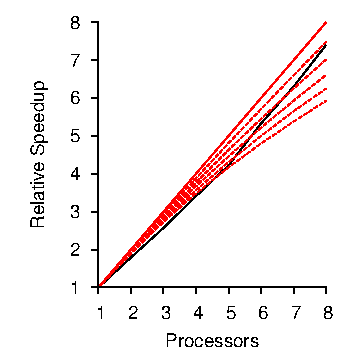
\includegraphics{figures/toolkit/speedup/speed}
\caption[Parallel speedup for toolkit code]{
\label{fig:toolkit:parallel}
Plot of relative speedup against number of processors for a two dimensional
simulation using the toolkit performed on horace.
The relative speedup obtained is plotted in a solid black line.
The solid red line represents ideal (1:1) speedup.
The five dashed red lines represent the speedup predicted for, from top to
bottom, $P = 0.99, 0.98, 0.97, 0.96, 0.95$.
The speedup obtained on 8 processors is very close to that predicted for a
parallel fraction of 0.99.
}
\end{figure}

\section{Experimental Protocols}
\label{sec:toolkit:protocols}

The toolkit developed provides a number of experimental protocols to use with
the cellular models to quantify the electrophysiological behaviour of the
modelled cells.  The provided protocols include the action potential duration at
90\% repolarization (\apd) and the action potential (AP) profile; the \apdr\ and
\apdr[50]\ restitution; the effective refractory period (ERP) restitution
(ERP\emph{r}); the conduction velocity (CV) restitution (CV\emph{r}); the
temporal vulnerability window to unidirectional conduction block (VW); the
threshold of excitation and a flexible system for specifying two dimensional
sheet experiments, including the initiation of re-entry via wavebreak protocols
and computation of the spatial vulnerability window.

\subsection{Action Potential}

\begin{figure}
\centering

\includegraphics{figures/toolkit/illustrations/labelled_ap_profile}
\caption[Illustration of AP properties]{
\label{fig:toolkit:illus:ap}
Schematic AP with various action potential properties noted.
Shown are the overshoot (OS), \apd, \apd[50], $\frac{dV}{dt}_{\text{max}}$ and
the resting membrane potential.
}
\end{figure}

The action potential profile is one of the fundamentals of cellular modelling,
with a number of associated properties, illustrated in
figure~\ref{fig:toolkit:illus:ap}.  These include the action potential
duration at 90\% repolarization, \apd; the action potential
duration at 50\% repolarization, \apd[50]; the maximal overshoot, OS; the
upstroke velocity, $\frac{dV}{dt}_{\text{max}}$ and the resting membrane
potential.

To compute these quantities, the cell is paced $N$\ times at given S1 interval.
After another S1 interval, a final AP is elicited from the cell and the
properties are measured.  In addition, it is common to want current and
cellular model state traces over the course of an AP and these can be provided
by the library alongside the membrane potential trace.

\subsection{Action Potential Duration Restitution}

The library calculates the APD\emph{r} via a standard S1--S2 protocol used in both
numerical simulations~\cite{Kim2002,Xie2002,Qu1999,Cherry2004,Cherry2007,Decker2009} and also in physiological
experiments~\cite{Boyett1978,Taggart1996}.  The APD\emph{r} is used
as a measure of how the cell responds to stimulations at different rates.

A single cell protocol to evaluate the ADP\emph{r}\ curve as results gained are
similar to strand protocols~\cite{Xie2002,Decker2009}\ with much less effort .
The cellular model is paced $N-1$\ times with a stimulus close to the threshold
value at a given stimulus interval, S1.  At this point, the state is saved for the
paced cells.  The $N$th S1 stimulus is then given, followed by the S2 after a
varying DI, which is reduced via an adaptive step to record the relationship
between DI and the APD of the following AP.  The toolkit also determines useful
parameters such as the maximal slope of the restitution curve, which can be
related to the stability of spiral waves within the tissue.  Both the \apdr\ and
the \apdr[50]\ restitution can be calculated.

\subsection{Effective Refractory Period Restitution}

The ERP\emph{r} is calculated by the library using standard experimental
protocols~\cite{Workman2001,Kharche2008}.
The ERP is defined as the shortest possible stimulus interval, S2, which still
allows a successful AP to be elicited after pacing $N$ times at a pacing
interval S1.  A successful AP is defined as an AP which has an amplitude
of at least 80\% of the magnitude of the preceeding AP.  
The rate dependence of the ERP is evaluated at a decreasing S1 interval.

To find the ERP for a given S1 interval the cellular model is paced $N$ times
at that interval.
The state is saved just before the $N-1^{\text{th}}$ AP is initiated.
The ERP is found via binary search.
The low guess for S2 is typically chosen as zero, whilst the high guess is the
S1 interval being tested.
The S2 interval for each attempt is the average of the high and low guesses.
After the state has been saved, the $N^{\text{th}}$ AP is initiated and its
amplitude recorded.
Then \ms{S2} after, the test AP is evoked.
After the test AP has been allowed to run its course, the amplitude is tested
and used to guide the next binary iteration.
Details of the elicited APs, such the S1 and S2 amplitudes and durations are
stored.
The binary iteration proceeds until the desired accuracy has been attained.

The reduction in S1 interval is stepped via an adaptive mechanism which is
used to keep the reduction in ERP between successive S1 intervals to below
\ms{1}.  The S1 interval is reduced until it is sufficiently short that the
S2 interval would fall within the $N^{\text{th}}$ AP.

\subsection{Vulnerable Window}

The VW measurement is based around a 1D ring model of cardiac tissue.
It is used to quantify the vulnerability of cardiac tissue to the genesis of
arrhythmia via re-entrant activity~\cite{Quan1990,Zhang2003,Gonzalez2003}.
The VW is defined as the time period in the refractory tail of a propagating
excitation wave that results in unidirectional conduction block.
In the case of a ring model of the tissue this causes retrograde propagation,
which forms a re-entrant excitation which cycles endlessly.
If the stimulus is given too early, then the tissue will still be refractory in
both directions and no propagation of excitation will ensue.
If it is given too late, then propagation will occur in both directions, which
in the ring case, results in the two excitation wavefronts annihilating each
other.
Normal pacing could then resume.
These three cases are illustrated in figure~\ref{fig:toolkit:illus:vw}.


\begin{figure}
\centering
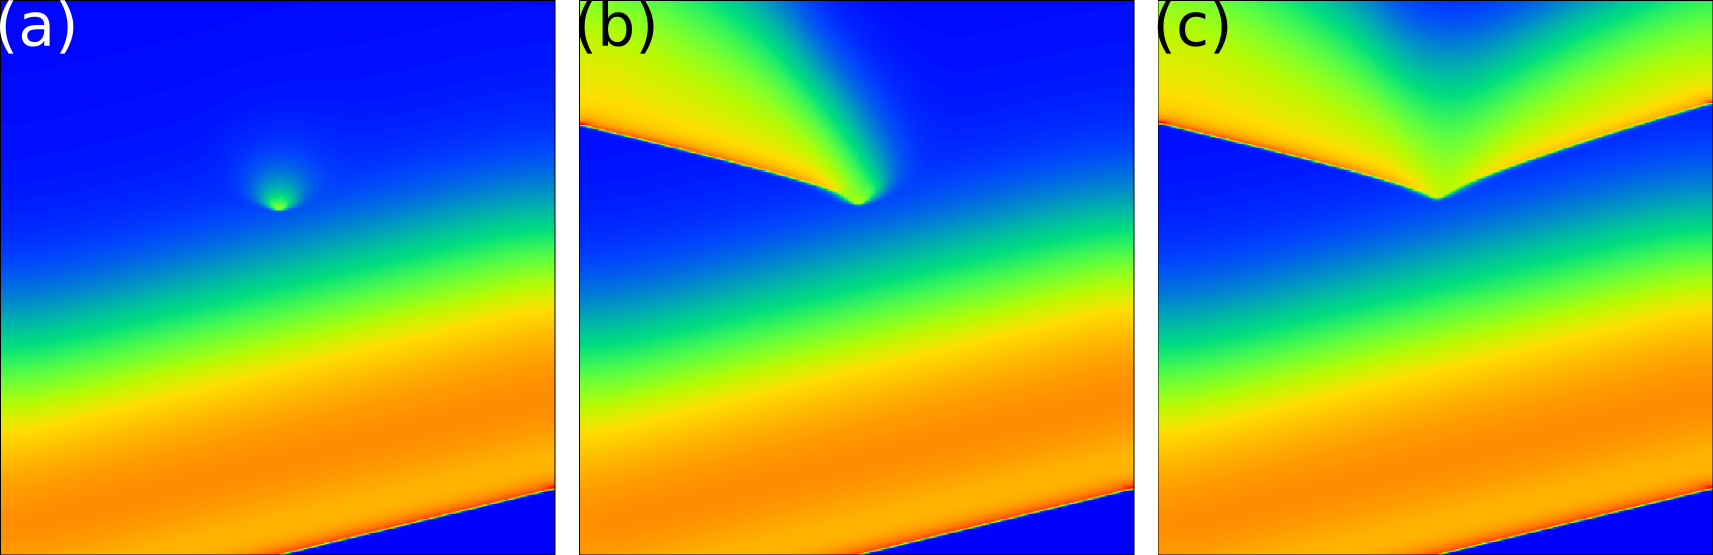
\includegraphics{figures/toolkit/illustrations/vw}
\caption[Illustration of VW cases]{
\label{fig:toolkit:illus:vw}
Illustrative space--time plots of the vulnerable window.
In all plots, colour represents membrane potential from resting (blue) to
depolarized (orange), position along the strand changes horizontally, whilst
time advances upwards.
Normal conduction is from left to right.
In all plots, the latter half of the last S1 pulse can be seen in the lower
right.
(a) Complete Block.  The stimulus is too early, and no excitation can be evoked.
(b) Unidirectional Block.
The stimulus has been delivered in the vulnerable window.
The stimulus can propagate only back along the strand.
In a ring, this would be re--entrant.
(c) Bidirectional Conduction.
The stimulus is delivered too late.
The bidirectional waves will anihilate each other.
}
\end{figure}


The VW is found in a 1D strand model, set up as described previously.
The use of a open-ended strand, not a connected ring, makes pacing the strand
easier, but does not effect the results.
The strand is 300 units long and with a space step of \mm{0.1}.
The strand is first given $N$ S1 conditioning stimuli which are administered to a
3 node (\mm{0.3}) section at the start of the strand.
Typically an S1 interval of \ms{1000}\ is used with 10 S1 pulses.
The test S2 stimulus is administered to a 4 node (\mm{0.4}) section, normally
centred in the middle of the strand, \ms{S2}\ after the $N^{\text{th}}$
conditioning excitation wave has passed the S2 stimulus site.
To reduce the computation time, the state is saved at this point.
The low guess for the binary iteration is chosen as \ms{0}\ and the high guess
as the S1 interval.
To judge the success of the S2 stimulus, the ends of the strands are watched for
successful excitation.
If there are no excitation waves crossing the ends after the $N^{\text{th}}$
excitation wave has passed, then it is in the region of total conduction block.
If one excitation wave crosses the end, it is in region of unidirectional block.
When two excitation waves cross the end, it is in the region of bidirectional
conduction.
The timing of the S2 stimulus is controlled via binary search, first to find the
boundary of total conduction block and unidirectional block and then to find the
boundary between unidirectional block and bidirectional conduction.
A minor optimisation above the usual binary search algorithm is possible in this
case, as a search for one boundary can be used to refine the range for the
second boundary too.

\subsection{Threshold of Excitation}

The threshold of excitation is a theoretical measure, proposed by Zhang et
al.~\cite{Zhang2003}\ and used in modelling studies~\cite{Kharche2008}.  It is
defined as the minimum stimulus current which, when delivered to a cell, will
cause the cell to depolarize to a membrane potential of at least \mv{-20}.  The
threshold of excitation is calculated for a range of stimulus intervals,
successively reducing the interval until it is impossible to elicit a
depolarization of sufficient magnitude.  At each stimulus interval it is
recorded if the test pulse elicits bidirectional, unidirectional or no
propagation.

The threshold of excitation is found in a 1D strand model.  The strand is 300
units long, with a space step of \mm{0.1}.  The strand is first given $N$ S1
stimuli at a rate which allows the strand to recover between each excitation
wave.  Each S1 stimulus is delivered to the first 4 nodes (\mm{0.4}) and is
chosen to be above the threshold of excitation.  The threshold of excitation is
calculated at the 100th node and so as this node depolarises, the state for the
whole strand is cached.

The threshold of excitation is then found via binary search, with a lower bound
of \unit{0}{nS} and an upper bound chosen to be 5x the normal threshold.  The
test stimulus is delivered $\Delta t$\ seconds after the 100th node depolarises
to a group of 4 nodes centred on the 100th node.  After the test stimulus is
delivered the 4 nodes are tested for the excitation condition, attaining a
membrane potential of \mv{-20}.  If it is successful, the current stimulus
strength will be assigned to the high guess.  If not, to the low guess.  In
addition, the simulation is continued to evaluate whether bidirectional,
unidirectional or no conduction of the excitation wave is evoked by the
stimulus.  The strand is then reset to the cached state and the new stimulus
strength is tested until a sufficient accuracy has been attained.  Once the
threshold of excitation has been determined for a given $\Delta t$\ the state of
the strand is once more reset to the cached state and a shorter $\Delta t$\
tested.

\subsection{Conduction Velocity Restitution}

The CV is the rate of propagation of the excitation wave.
It is determined by the difference in excitation times at two points divided by
the distance between them.
It is measured both in both experimental and numerical studies and is therefore
useful in validating experimental results.
A related measurement is the minimum conduction interval.
The minimum conduction interval is the shortest interval between an S1 and S2
stimulus which still propagates successfully.
It is similar to the ERP, but can also be influenced by inter-cellular coupling
and heterogeneity in the strand.
The CV\emph{r} is found via stimulating the strand at successively shorter
intervals and noting the changes in the measured
CV~\cite{Cherry2008,Zhang2003,Qu2006}.
The minimum stimulus interval is found via noting when the curve ends.


The CV\emph{r} is found in a 1D strand model, set up as described previously.
The strand is 300 units long with a space step of \mm{0.1}.
Stimuli above the stimulus threshold are delivered to a 4 unit (\mm{0.4}) length
at one end of the strand.
The strand is first given $N$ S1 stimuli.
Typically an S1 interval of \ms{1000}\ is used with 10 S1 pulses.
The S2 stimulus is then delivered \ms{S2} seconds later.
The CV is estimated from the difference in excitation times, defined as the
instant at which the node is excited above \mv{-60}, at 2 nodes which are
located 100 nodes apart.
This minimizes any possible influence from boundary conditions.
The S2 time is then stepped until a second excitation wave
does not propagate the length of the strand.


\subsection{Spiral Wave Dynamics}

The dynamic behaviours of spiral waves are characterised by the stability,
mobility and lifespan (LS).
Spiral Wave LS is examined experimentally~\cite{Kumagai1997} and
numerically~\cite{Qu2000,Nygren2001,Cherry2007,Clayton2005,Zhang2003}.
The LS of the spiral wave and the meander pattern of the tip are both used to
gain insight into the behaviour of the tissue under conditions of cardiac
arrhythmia.

Spiral waves are initiated in a square sheet of tissue $375\,\text{x}\,375$
nodes in dimension with a space step of \mm{0.1}, as described previously.  The
tissue is first stimulated along one edge via a stimulus current applied to a
row of nodes extending the length of the tissue and 3 nodes (\mm{0.3}) in width.
The planar wave is then allowed to propagate over the tissue.  Some time after
the first wave is initiated, a second stimulus is applied.  The second stimulus
is applied to half the tissue, bisecting the propagation front of the first wave.
The second stimulus is a voltage clamp, with all the included tissue clamped to
a `high' potential, typically \mv{+0} for a millisecond.  The
generated spiral is then allowed to evolve until it self-terminates, the spiral
wave tip exits the tissue or until a sufficient amount of time has passed such
that the spiral can be classified as `persistent'.  The time allowed for a wave
to be classified as persistent is typically 5 or \unit{10}{s}.

The spiral wave tip traces are calculated via a standard contour based
algorithm, comparing the \mv{-60} contour line on snapshots of the electrical
activity \ms{2.5} apart.

\subsection{Spatial Vulnerability of Cardiac Tissue}

The spatial vulnerability (SV) of cardiac tissue is defined as the smallest
length of tissue which, when given a stimulus at the threshold level in the wake
of a propagating wave, gives rise to at least one `figure of eight'
re-entry~\cite{Zou2005}.
A figure of eight re-entry occurs when the excitation waves from the ends of the
test length propagate back through the centre of the length.
This results in a pair of contra-rotating spiral waves, one at each end of the
test length.
The SV is useful for quantifying a mutation or condition's potential for
arrhythmogenesis by giving an indication of the size of ectopic focus required
to excite the tissue.
A small SV indicates that the tissue could be very likely to have arrhythmic
episodes.

The sheet model used for the determination of the SVW can vary in size, as the
SVW can vary substantially, depending on the electrophysiology being simulated
by the cellular models at the nodes, but the smallest used is typically
$375\,\text{x}\,375$ nodes, with a spatial resolution of \mm{0.1}.  The sheet is first given one
conditioning excitation, initiated by injecting a strip of nodes 3 nodes
(\mm{0.3}) in width with current along one edge of the sheet.  The wave is then
allowed to propagate through the tissue.  When the VW of the tissue is
positioned at the centre of the tissue, the test stimulus is delivered.  The
test stimulus is an area of tissue 20 nodes (\mm{2}) wide and of variable length.
After the test stimulus is delivered, the sheet is observed until figure of
eight re-entry is observed, or it is obvious that it will not occur.  The
protocol is then repeated with a test stimulus area of greater length.


\section{Results From Simulation Studies}

The cardiac simulation toolkit has been used in several simulation studies.
Here I present two such studies, representing different aspects of the toolkit.
The first is based on an experimental study which determined the existence of a
novel ion channel in the human atrium which caries an anion current through the
cellular membrane.  The second is principally a 2D study, concerning the effects
of Atrial Fibrillation induced Electrical Remodelling (AFER) and
electrophysiological heterogeneity in a 2D idealization of the right atrium and
the sino-atrial node.

\subsection{Anion Currents In The Human Atrium}

In a recent experimental study, Li et al.~\cite{Li2007} determined the existence
of a novel outwardly rectifying anion current in human atrial myocytes isolated
from right atrial appendages taken from patients undergoing coronary bypass
surgery.
A preliminary computational study has been conducted~\cite{Li2007}\ to
investigate the effects of the anion sensitive current, \ii{ANION}, on atrial
action potentials.
However it is still unclear on how this novel current affects intra-atrial
excitation conduction.
This section aims to investigate in detail the effects of \ii{ANION}\ on atrial
action potential, conduction behaviours and the dynamic behaviours of re-entrant
spiral waves.

The Li et al.~\cite{Li2007}\ study determined the current carried by this novel
ion channel, \ii{ANION}, could be modelled by
\begin{equation}
\label{eqn:anion:ianion}
I_{ANION} = g_{ANION} \frac{V-E_{ANION}}{1-\left(c\times e^{d\times\left(V-E_{ANION}\right)}\right)}
\end{equation}
where $g_{ANION}$ is the conductivity of the anion channel, $E_{ANION}$ is
the reversal potential of the channel and $c$ and $d$ are constants to
describe the behaviour.
All other symbols have their usual meanings.
They presented two sets of parameters for (\ref{eqn:anion:ianion}) given in
table~\ref{tbl:anion:params}, which described the current through the channel
when carrying a majority of \nothree\ or $\text{Cl}^{\text{-}}$ ions.

\begin{table}
    \caption[Parameter sets for the anion carrying current]{
        Parameter sets for the anion sensitive current \ii{ANION}\ when carrying
        \nothree\ and $\text{Cl}^{\text{-}}$\ ions.
    }
    \begin{tabular}{ l  c c}
    \toprule
    & \nothree & $\text{Cl}^{\text{-}}$ \\
    \midrule
    $g_{ANION}$ & 0.37   & 0.19 \\
    $E_{ANION}$ & -45.64 & -45.64 \\
    $c$         & 0.87   & 0.94 \\
    $d$         & $8.4\,\text{x}\,10^{\text{-4}}$ & $2.5\,\text{x}\,10^{\text{-4}}$\\
    \bottomrule
    \label{tbl:anion:params}
    \end{tabular}
\end{table}

This simulation study used the parameter set for the anion current carrying
$\text{Cl}^{\text{-}}$ ions.
The effects of the addition of this current to atrial myocyte cells was
quantified.
In the following paragraphs, `control' is used to denote the original
Courtemanche~et~al.~\cite{CRN98}\ atrial myocyte model and `anion' to denote the
Courtemanche~et~al. model with the addition current described by
(\ref{eqn:anion:ianion}) and using the $\text{Cl}^{\text{-}}$ parameter set from
table~\ref{tbl:anion:params}.

\subsubsection{Methods}

The effect on the behaviour of the cells caused by the anion current was
quantified using the simulation library described previously in this chapter for
control and anion cases.
As this simulation study was based on the CRN cell, the standard stimulus was
\ms{2} in duration and \unit{2}{nS} in magnitude.
Unless an alternative protocol is mentioned, all simulations directly followed
those described in Section~\ref{sec:toolkit:protocols}.

Simulating a single cell, the following measures were quantified: the AP
profile, the restitution of APD at 50\% repolarization, \apdr[50], the
restitution of APD at 90\% of repolarization, \apdr\ and the Effective
Refractory Period restitution, ERP\emph{r}.  The maximal fast sodium activation
was quantified at the same time as the \apdr\ was computed and is the product of
the three gates in \ii{Na}, as $m^{3}hj$. In all the single cell cases, the
cell was paced 10 times before the measurement was taken, to allow simulation
parameters to settle and to adapt to any changes in pacing rate.  Storage of the
cellular state was used in all appropriate points in the simulation, to minimise
computational time.

Using a 1D strand model the temporal Vulnerability Window to unidirectional
conduction block, VW, the Conduction Velocity restitution, CV\emph{r}\ and the
threshold of excitation were computed.  The strand model used was 300 nodes long
and had a space step of \mm{0.1}.  The diffusion coefficient, $D$, was set to
$0.03125\,\text{mm}^{\text{2}}\,\text{ms}^{\text{-1}}$~\cite{Biktasheva2005}.
In all 1D simulations the strand was paced 10 times before measurement was
taken.  In all simulations this state was then cached and restored as
appropriate, as described in the algorithms section of this chapter.

Using a 2D tissue model the lifetime of re-entrant spiral waves was estimated,
following the wave-break protocol outlined earlier.  The sheet had dimensions of
$375\times375$ nodes and a space step of \mm{0.1}.  The clamp potential used
to break the wave was \mv{0} and it was applied for \ms{1}.

\subsubsection{Results}


\begin{figure}
\begin{center}
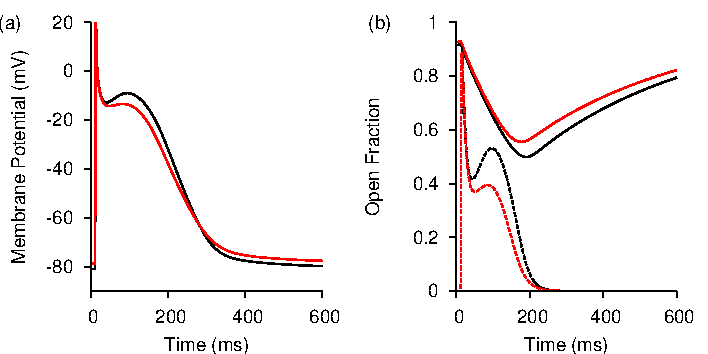
\includegraphics{figures/toolkit/anion/figures/01_AP}
\end{center}
\caption[Anion Current AP Profiles and \ii{Ca,L}\ gating parameters]{
\label{fig:tookit:anion:ap}
(a) AP profile for the CRN model in control (black) and anion (red) cases.
The inclusion of the $\text{Cl}^{\text{-}}$ carrying current results in a small
change of AP morphology, with a depressed plateau potential and an elevated
resting potential.
(b) Fractional opening of the gates of \ii{Ca,L}.
The $d$ (activation) gate is shown dashed, the $f$ (inactivation) gate solid.
Colours as in panel (a).
The $f$ gate takes longer to inactivate, whilst the $d$ gate does not activate
as much.
}
\end{figure}

The AP generated by the control and anion simulations are shown in
figure~\ref{fig:tookit:anion:ap}(a).
The \apd\ is slightly reduced from \ms{299.6} to \ms{297.3}, whereas the
\apd[50]\ is more significantly reduced, from \ms{180.1} to \ms{158.1}.
The AP profile shows a depressed plateau region (phase 2), reduced from
\mv{-9.56}\ to \mv{-14.1}\ and a slightly elevated resting potential,
\mv{-79.0}\ in the anion case cf. \mv{-80.9}\ in control.
This is consistent with the Li~et~al.~\cite{Li2007} study, and is included here
only for completeness.

Transients of the $d$ and $f$ gate of the \ii{Ca,L}\ open fractions are shown in
figure~\ref{fig:tookit:anion:ap}(b).
The $f$ gate in the \ii{ANION}\ case has a higher fraction of open channels for
longer than the control case.
The $d$ gate does not activate as much in the plateau region, contributing to
the shorter plateau.


\begin{table}
\caption[Calculated parameters for anion and control cells]{
\label{tbl:toolkit:anion_params}
Various calculated parameters for control (original CRN cell) and anion (CRN
cell modified to include $\text{Cl}^{\text{-}}$-carrying current).
The duration of the action potential at 50\% and 90\%
repolarization, \apd[50]\ and \apd\ respectively.
The maximum observed upstroke velocity of the action potential,
$\frac{dV}{dt}_{max}$.
The temporal vulnerability window to unidirectional conduction block, VW.
}
\begin{center}
\begin{tabular}{r l l l l}
\toprule
Case & \apd\ (ms) & \apd[50]\ (ms) & $\frac{dV}{dt}_{max}$ ($\text{mV}\,\text{ms}^{\text{-1}}$) & VW (ms)  \\
\midrule
Control & 299.6 & 180.1 & 217.1 & 3.22 \\
Anion & 297.3 & 158.1 & 210.6 & 3.94 \\
\bottomrule
\end{tabular}
\end{center}
\end{table}

The computed APD\emph{r}\ curves under the control and anion conditions are shown
in figure~\ref{fig:tookit:anion:apdr}(a) and \ref{fig:tookit:anion:apdr}(b), for the
restitution curves of APD at 50\% (\apdr[50]) and 90\% (\apdr) of repolarization,
respectively.
The
\apdr[50]\ shows the most significant differences, with the anion
curve depressed by \ms{20} even at the largest DI, increasing to a maximum
difference of over \ms{40} at at DI of \ms{380}.
The two curves then cross over at a DI of \ms{200}.
The \apdr\ curves, by contrast, are very similar for control and anion cases at
large (over \ms{600}) DI.
Between \msrange{100}{400}\ DI, the anion case is depressed compared to the control
case, with a difference of up to \ms{25}\ observed in the measured APDs.  At
\ms{100}, the curves rejoin one another and show a rapidly increasing slope as the
DI approaches \ms{0}.

\begin{figure}
\begin{center}
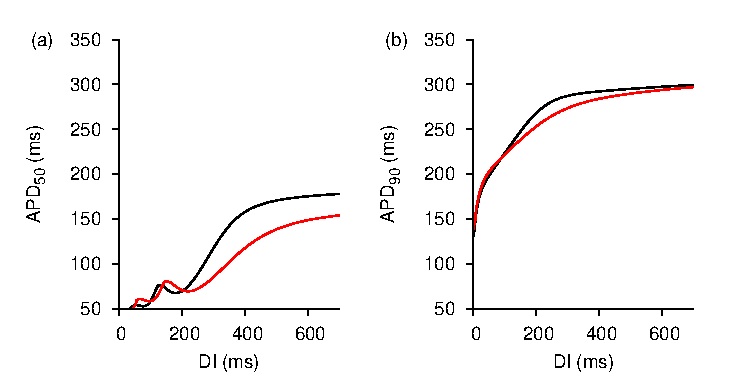
\includegraphics{figures/toolkit/anion/figures/02_APDR}
\end{center}
\caption[Anion Current APD Restitution]{
\label{fig:tookit:anion:apdr}
(a)
\apdr[50] curves for the CRN model in control (black) and anion (red) cases.
The two variants are different for all the DI in the simulation,
with the anion case below the control case for much of the DIs.
The slope is reduced by \ii{ANION}, compared to
the control case.  The curves cross at DI \ms{200}.
(b)
\apdr curves for the CRN model in control and anion cases.
The two variants behave the same at large DIs, but at decreasing DI the
anion case shows a greater reduction in the \apd.
At short DI (below \ms{100}) the two curves rejoin each other.
}
\end{figure}
\begin{figure}
\begin{center}
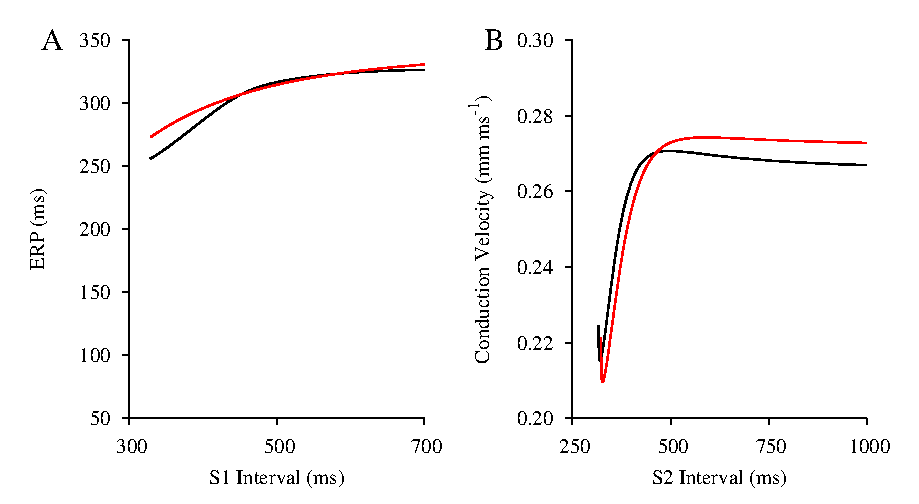
\includegraphics{figures/toolkit/anion/figures/03_ERPR}
\end{center}
\caption[Anion Current ERPr and CVr] {
\label{fig:toolkit:anion:erpr}
(a)
ERP\emph{r} curves for the CRN model in control (black) and anion
(red) cases.
The addition of the \ii{ANION} current changes the behaviour of the cell from a long
and flat plateau region followed by a relatively sharp decrease into a more
constant decline.
(b)
CV\emph{r}\ curves for the CRN model in control and anion cases.
 The CV\emph{r}\ curves are relatively flat for both cases over the range of
\msrange{500}{1000}, before they decrease rapidly in CV until the minimum
S2 interval is reached at approximately \ms{320}.
The CV is higher for the anion case at longer S2 intervals, before it
falls below control at an approximate S2 interval of \ms{460}.
}
\end{figure}

The ERP\emph{r} curves produced by the control and anion cases are shown in
figure~\ref{fig:toolkit:anion:erpr}(a).
In both cases the ERP\emph{r}\ curves are relatively
flat, decreasing by approximately \ms{60}\ over the \ms{700}\ range of S1
intervals considered.  The addition of the \ii{ANION}\ current changes the
behaviour of the ERP\emph{r} curve in a manner which is not simply a shift left
or right.  The control case shows a response which has a clear plateau region
which continues until an S1 interval of \ms{500}\ is reached and then a
relatively steeper decline until eliciting an AP of the appropriate magnitude
becomes impossible at an S1 interval of \ms{330}.  The anion case, by contrast,
shows a decreasing ERP over the whole range of S1 intervals considered although
it too shows its steepest slope just before eliciting a sufficiently large AP
becomes impossible, also at approximately \ms{330}.  At long S1 intervals (above
\ms{700}) the ERP\emph{r}\ is longer for the anion case before the curves cross
at \ms{600}\  and then again at \ms{450}\ with the ERP in anion at the point
where further stimulation becomes impossible almost \ms{20}\ higher than in the
control case.

The temporal VW increased with the addition of the anion current from \ms{3.22}
in control to \ms{3.94}\ in anion case, a 22\% increase in the size of the
region of unidirectional conduction block, shown in table~\ref{tbl:toolkit:anion_params}.
The CV\emph{r}\ curves, shown in
figure~\ref{fig:toolkit:anion:erpr}(b), suggest that tissue with the anion sensitive current
shows faster CV at normal physiological stimulus intervals (corresponding to
\msrange{500}{1000}).
The average conduction velocity with \ii{ANION}\ is
$0.274\,\text{mm}\,\text{ms}^{\text{-1}}$ in anion,
compared with $0.268\,\text{mm}\,\text{ms}^{\text{-1}}$ in control in this range
of S2 intervals.
As the conduction interval is reduced below \ms{500}, the conduction velocity
starts to decrease rapidly until conduction stops at \ms{323.4} for anion and
\ms{317.1} for control.
There is a brief recovery of conduction velocity visible in both cases, just
before conduction block.

\begin{figure}
\begin{center}
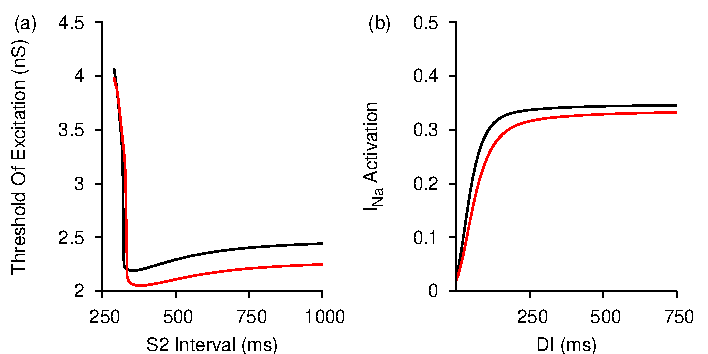
\includegraphics{figures/toolkit/anion/figures/04_ToE}
\end{center}
\caption[Anion Sensitive Threshold Of Excitation and \ii{Na} activation]{
\label{fig:toolkit:anion:toe}
(a)
Threshold of excitation curves in control (black) and
anion (red) cases.
As S2 decreases, so does the threshold of excitation until a critical point is
reached and the current which must be injected to reach the threshold almost
doubles.
In the control this comes at a $\Delta t$ of
\ms{321}\ and in anion at \ms{330}.
Until the critical point threshold of excitation is consistently lower for cells
with \ii{ANION}\ present.
(b)
Maximal activation of the fast sodium current, \ii{Na}, as DI is decreased.
The fast sodium current consistently activates to a greater degree in control
cases.
The effect is rate dependent with the greatest difference observed at DI \msrange{150}{200}.
}
\end{figure}

The threshold of excitation, shown in figure~\ref{fig:toolkit:anion:toe}(a), shows that
\ii{ANION} reduces the minimum stimulus current by approximately \unit{0.2}{nS},
a reduction of 10\%, at almost all $\Delta t$\ intervals.  It is also
interesting to note that both control and anion tissue types show `supra-normal'
excitability, with the minimum stimulus current decreasing as $\Delta t$\
decreases.  This occurs until a critical point is reached when the cell suddenly
becomes significantly harder to excite, with the minimum stimulus current
increasing almost 100\%.
This occurs \ms{9}\ later in control tissue at
\ms{321}\, compared with \ms{330}\ in control.

The maximal activation of the fast sodium current, \ii{Na}, is shown in
figure~\ref{fig:toolkit:anion:toe}(b).
The presence of \ii{ANION}\ consistently reduces the maximal activation of \ii{Na}.
At long DI, greater than \ms{400}, the reduction is 3\%, increasing to almost
twice that in the range of \msrange{150}{200}.
Both curves rapidly decrease to almost no \ii{Na}\ activation at an DI of
\ms{0}\ but the anion case starts this descent first.
\begin{figure}
\begin{center}
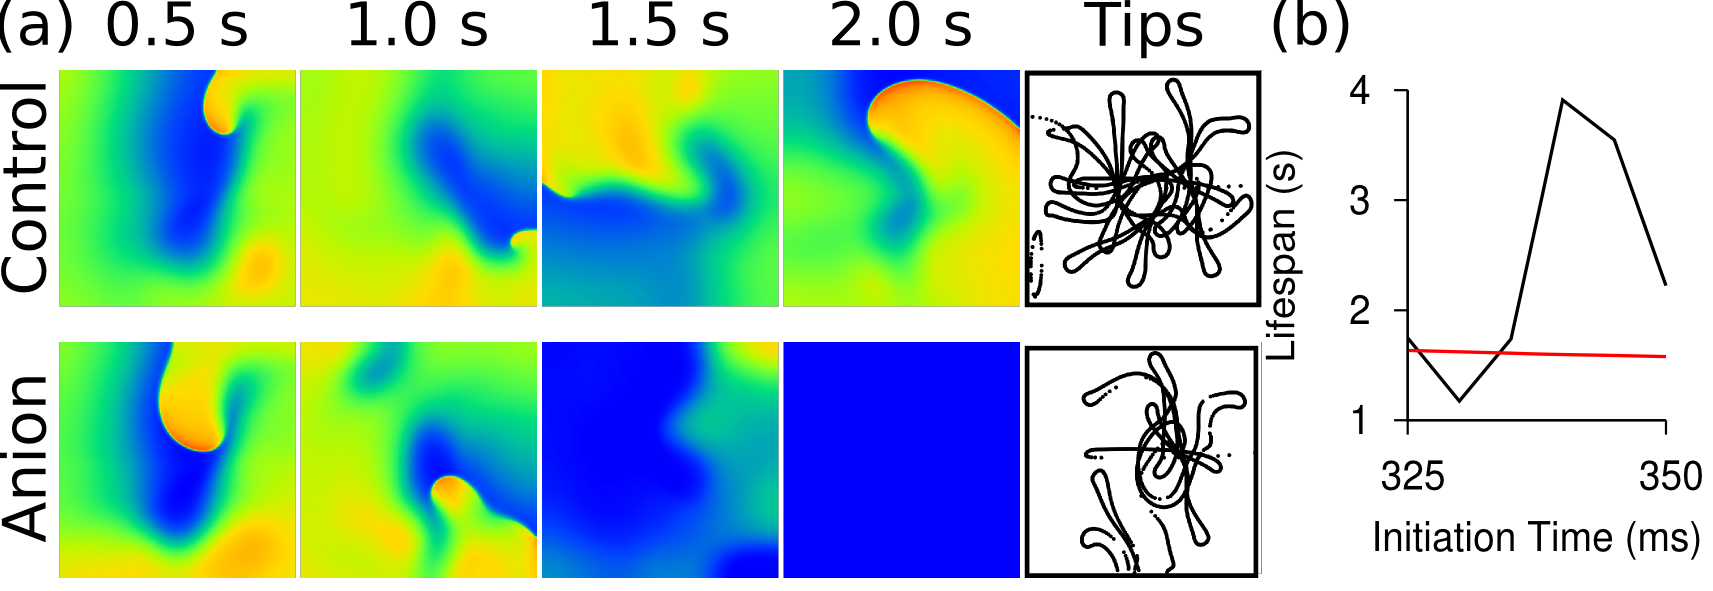
\includegraphics{figures/toolkit/anion/twod_traces}
\end{center}
\caption[Anion Sensitive Tissue Sheets and Spiral Lifespands]{
\label{fig:toolkit:anion:spiral}
(a)
Representative membrane potentials and tip trace for control (top row) and anion
sensitive cases (bottom row).
Times are from the initiation of spiral activity via cross--field protocol.
Cross--field stimulus was delivered at \ms{345}\ wall time.
Colour represents membrane potential and is coloured from blue (depolarised,
\mv{-80}) to orange (excited, $>\mv{0}$).
Both spiral waves are highly mobile, meandering over a very large area of
tissue.
(b)
Lifespan as related to time of initiation.
Lifespan in \ii{ANION}\ is relatively constant at around \ms{1600}\ whilst
control lifespan fluctuates considerably.
}
\end{figure}
Spiral waves were induced in a square sheet.
Representative plots of the
membrane potential over the whole sheet, produced as the simulation was ongoing,
are shown in figure~\ref{fig:toolkit:anion:spiral}(a).
The top row corresponds to control tissue, whilst the bottom row has an
\ii{ANION}\ sensitive current active.
Times of the membrane potential snapshots are relative to initiation of reentry at t = \ms{345}.
Tip traces are in the 5th column.
In both cases the spiral wave starts in the centre of the tissue and then follows a
looping track around the tissue before finally it exits the tissue when it
cannot turn fast enough around its own refractory tail.
Lifespans of reentry from differing initiation times are shown in
~\ref{fig:toolkit:anion:spiral}(b).
Lifespan in \ii{ANION}\ is relatively constant at around \ms{1600}\ whilst
control lifespan fluctuates considerably, from \ms{1175}\ to \ms{3910}.

\subsubsection{Discussions and Conclusions}

The effects of the inclusion of an anion sensitive current do not seem to be
that large, at least when considered on the single cell level.
However, despite the small influence of the current on the action potential duration,
it does have significant effects on the restitution properties of the cell and
on the behaviour of cells in a tissue.
The general behaviours of the Courtemanche cell have been discussed elsewhere,
for example in~\cite{CRN98,Cherry2008a}, I only discuss the differences the
\ii{ANION}\ current makes.

The most noticeable effect of the inclusion of \ii{ANION}\ in a cellular model
is the abbreviation of the \apd[50]\ and an accompanying reduction in the
plateau potential.  The abbreviation is due to \ii{ANION}\ acting as a
rectifying current when the membrane potential is above \mv{-45}.   Conversely,
at potentials below \mv{-45}\ \ii{ANION}\ acts to depolarize the cell, leading
to the slightly elevated resting membrane potential observed between action
potentials.  This difference in effect is what leads to the interesting
behaviours observed in cells with \ii{ANION}.

The \apdr[50]\ and \apdr\ curves show that \ii{ANION} has a rate dependent
effect.  Both curves are flattened in the cells which include \ii{ANION}\, but
this flattening is not uniform over the range of DIs considered.
\ii{ANION}\ has a simple exponential dependence on the membrane potential and no
time-dependent gating variables however, so it is not \ii{ANION}\ that causes
this rate dependence directly.
Instead, we must look to the currents active within the plateau region of the
action potential.
\ii{CaL}\ is the principle current responsible for the plateau region of the
action potential and unlike \ii{ANION} it has both time and voltage dependant
gating variables for activation, $d$, and inactivation, $f$.
The $d$\ gate is not as interesting as the $f$\ gate, as its time-course is not
affected by the presence of \ii{ANION}, although its activation during the
plateau region is reduced.
However, the $f$\ gate in \ii{ANION} cells never inactivates as completely as
it does in the control simulations which lack the current.

For the 1D strand results, both the CV\emph{r} and threshold of
excitation data also show rate dependent influence.
At a long stimulus interval, the increased excitability of the cell by the anion
current leads to a higher conduction velocity~\cite{Nygren2000}.
The increased excitability at long stimulus interval is due to the inward nature
of the anion current in the very first stages of the action potential.
This increased excitability allows atrial cells with \ii{ANION}\ to conduct the
excitation wave faster until, when the stimulus interval reaches a critical value of
\ms{500}, control cells start to conduct faster.
At this stimulus interval, the threshold of excitation is still lower for the
anion case, so another factor is responsible for the reduction in conduction
velocity.
The excitability of the cell is an important influence on the conduction
velocity, but it is not the only factor.
Another major factor is the upstroke velocity of the action potential which is principally
determined by the fast sodium current, \ii{Na}.
This is partially inactivated by the elevated resting potential in the anion
case, which also reduces the rate of recovery of the inactivation variables.
When the test stimulus is delivered after a reduced conduction interval in the
anion case \ii{Na}\ does not open as fully, slowing the upstroke and thus
leading to a reduced conduction velocity at short stimulus intervals, compared
with the control case.

The increase in the
vulnerability window appears to be quite significant, at over 20\% larger than
the vulnerability window in tissue without \ii{ANION}.
An increased vulnerability window has an obvious influence on the genesis of
re-entrant excitation---A larger vulnerability window increases the chance of a
premature excitation interrupting the normal function of the heart.
Though in both cases, the vulnerability window is relatively small.


Dynamic behaviours of the 2D spiral wave are interesting.
Both cells show a highly mobile spiral tip, due to their long \apd\ and ERP
relative to the size of the tissue.
However in the \ii{ANION}\ case, this does not translate into a widely varying
spiral lifespan, as might be expected from such mobility.
The restitution properties are generally slightly flattened by the inclusion of
\ii{ANION}, although perhaps importantly here, in the rapid pacing region, the
ERP is higher for \ii{ANION}\ bearing cells.
Further investigation, perhaps using the phase field
method~\cite{Biktashev1994}\ to start with a `stationary' spiral would be of use
to elucidate the effects.



\subsection{Atrial Fibrillation Induced Remodelling And Heterogeneity}

The human atria consists of several tissue types each with distinct
electrophysiological properties.  It has previously been shown that
inhomogeneity in tissues can lead to re-entrant activity
\cite{Bernus2005, Coronel1992, Kumagai1997}.  There is also experimental
data available on the ion channel remodelling due to atrial
fibrillation induced remodelling (AFER) during chronic atrial
fibrillation (AF) on human atrial cells~\cite{Bosch1999,Workman2001}.

In this study changes in electrophysiological
behaviour in cell and 1D homogeneous models under AFER compared to control
conditions were quantified.
Further, re-entrant waves in 2D electrically homogeneous
and electrically heterogeneous sheets were studied.

\subsubsection{Methods}

The human atrial action potential (AP) model by Courtemanche et
al.\cite{CRN98} was used in this study.  Modifications were
incorporated to reproduce the differing APs of the different atrial cell
types~\cite{Seemann2006}.  This produced distinct APs for the
crista terminalis (CT), pectinate muscles (PM), atrio-ventricular ring
bundle and the Bachmann bundle.  Atrial myocyte (AM) cells were modelled
by the original CRN model.

The data for AFER were taken from experiments by Bosch et
al.~\cite{Bosch1999} and Workman et al.~\cite{Workman2001}, representing
the changes in ion channels in patients after one month (Bosch)
and up to six months (Workman) of chronic AF, respectively.  The
modifications to the cellular electrophysiology were described in
Kharche et al.~\cite{Kharche2007}\ and reproduced in table~\ref{tbl:afer:params}.


\begin{table}
    \caption[Parameter modifications for AFER]{
       Parameter modifications to the unmodified CRN model to account for the
       electrophysiological remodelling of atrial myocytes.
       Two sets of parameter modifications are provided, to account for the
       experimental data collected by Bosch~et~al.~\cite{Bosch1999} and
       Workman~et~al.~\cite{Workman2001}.
       When percentages are given, they are up or down regulations compared to
       the magnitude of the current in the unmodified CRN model.
       The data from Bosch~et~al. also included at \mv{-16}\ shift in the steady
       state activation of \ii{to}\ and a \mv{+1.6}\ shift in the steady state
       activation of \ii{Na}.
    }
    \begin{center}
    \begin{tabular}{ l r r}
    \toprule
    Current & Bosch & Workman \\
    \midrule
    \ii{K1}   & $+235$\% & $+90$\% \\
    \ii{Ca,L} & $-74$\% & $-64$\% \\
    \ii{to}   & $-85$\% & $-65$\% \\
    \ii{Kur}  & --- & $+12$\% \\
    \ii{NaK}  & --- & $-12$\% \\
    $\tau_{\text{fCa}}$ & $+62$\% & --- \\
    \bottomrule
    \label{tbl:afer:params}
    \end{tabular}
    \end{center}
\end{table}

The effects of AFER were quantified through a variety of measures.  The
\apdr\ was calculated as described previously.
There were 10 S1 stimuli at a frequency of \unit{1}{Hz}, followed by a varying DI.
The ERP\emph{r} was calculated as described previously, with 10 S1 delivered at
the given pacing rate and then a final S2 stimulus was used to determine the ERP
after Workman et al.~\cite{Workman2001}.
The VW and the CV\emph{r} were determined for control,
Bosch and Workman conditions, for each of the three atrial cell types
considered.
There were therefore nine 1D strand models tested.  The strand
models were each 200 nodes long, with a spatial resolution of \mm{0.1}.  The
diffusion constant used for all simulations was set to
$0.03125\,\text{mm}^{\text{2}}\,\text{ms}^{\text{-1}}$~\cite{Biktasheva2005},
giving a solitary wave conduction velocity of
$0.267\,\text{mm}\,\text{ms}^{\text{-1}}$\ in control atrial tissue.  In all 1D
strand simulations there was 1 S1 pulse and one S2 pulse.  This pulse was
applied over 4 nodes (\unit{0.4}{mm}), had duration \ms{2} and magnitude
\unit{4}{nS}.
The higher stimulus strength was necessary to excite the AFER remodelled tissue.

Further, a 2D electrically heterogeneous sheet model was developed based on a
laboratory photograph of the right atrium.  The photograph was digitized at a
spatial resolution of \mm{0.1}. The model developed by segmenting areas of the
tissue into AM, PM and CT tissue types.  The complete model had an approximate size of
$130\times100\,\text{mm}$ and consisted of approximately 1 million active cell nodes.  The
simulations were performed with all cells under control, Bosch and Workman conditions,
with the conditions applied uniformly to the tissue.  All 2D sheet simulations
were performed with the space step of \mm{0.1} and a time step of \ms{0.05}.

\subsubsection{Results}

Simulations were performed for all three cases: control, Bosch and Workman.
However the results for Bosch and Workman were qualitatively similar, although
Bosch showed a much more profound effect on \apd\ reduction.

\begin{figure}
\centering
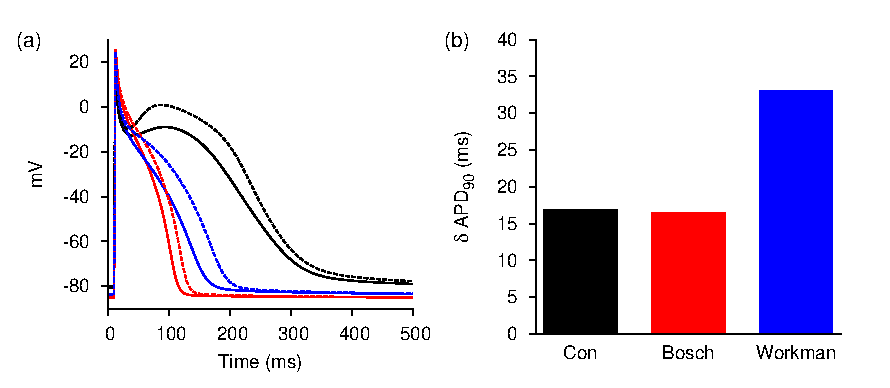
\includegraphics{figures/toolkit/afer/figures/01_APD}
\caption[AFER AP Plots And APD differences]{
\label{fig:toolkit:afer:apd}
(a).
Action potential profiles after pacing at \unit{1}{Hz}.
Results are shown for AM/PM cells (solid lines) and CT cells (dashed lines).
Control parameter traces are black, Bosch are red and Workman traces
blue.
The CT cells have a longer APD in all cases and show an elevated plateau
potential.
(b).
APD differences between AM/PM cells and CT cells after pacing at \unit{1}{Hz}.
Colour scheme as for panel (a).
There is almost no difference in $\delta$\apd\ between control and Bosch CT cells,
but $\delta$\apd\ increased markedly when Workman parameters are used.
}
\end{figure}

Incorporating the heterogeneity and AFER data causes significant differences in
\apd\ and AP morphology to manifest, as shown in
figure~\ref{fig:toolkit:afer:apd}(a).
The effects of AFER are not uniform across the different cell types of the
atrium in both cases (figure~\ref{fig:toolkit:afer:apd}(b)).
The difference in the AP between AM/PM myocytes and CT myocytes in the Workman
remodelled case is almost double that seen in either the Bosch remodelled case
or control case.
Note that in all cases there is almost no difference between AM and PM types.


\begin{figure}
\centering
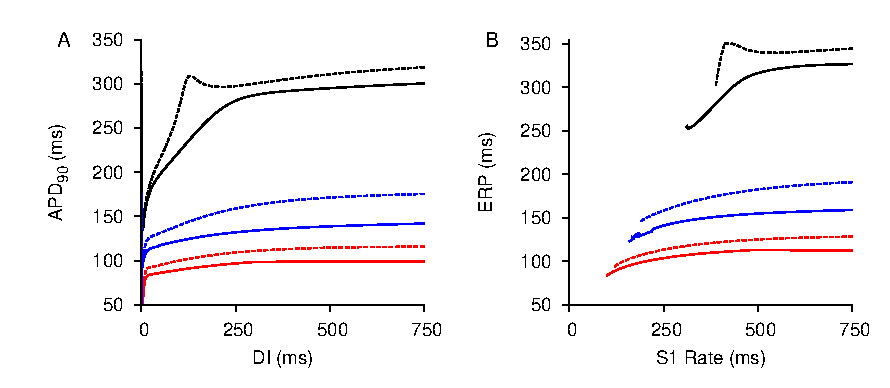
\includegraphics{figures/toolkit/afer/figures/02_APDR}
\caption[AFER APDr and ERPr curves]{
\label{fig:toolkit:afer:apdr}
(a)
\apdr\ curves showing \apd\ plotted against diastolic interval (DI) for control
(black), Bosch (red) and Workman (blue) cases.
AP/PM curves are shown as solid lines, CT curves are dashed.
AFER acts to flatten the restitution curves.
In all cases CT \apd\ is above AM/PM \apd.
(b)
ERP\emph{r}\ curves showing ERP plotted against S1 interval.
Colour scheme is as for panel (a).
In all cases CT ERP is above AM/PM ERP.
Note that AFER enables successful excitation at much lower S1 intervals.
}
\end{figure}

The \apdr\ curves, shown in figure~\ref{fig:toolkit:afer:apdr}(a), are
flatter over much of the range of diastolic intervals for Bosch and Workman as
compared to control.
The curves have two clear phases in the AFER cases; a very steep initial rise
and then slower, asymptotic rise in \apd.
In the control case the curves show an intermediate a phase with a slope between
the two extremes.
In the control CT case, the curves include a prominent notch at a DI of
approximately \ms{130}\ which is caused by the up regulation of \ii{Ca,L}\ in CT
cells.
The down regulation associated with the AFER removes this.
In both of the AFER cases, the curves are almost flat at DI \ms{750}, but in the
control case, the \apd\ is still rising.
The figure also emphasises the increased heterogeneity observed in the Workman
case.

In AF tissue, the ERP\emph{r} was flattened for all tissue types compared with
the control cells, as shown in figure~\ref{fig:toolkit:afer:apdr}(b).
The curves also extended to lower S1 intervals for AF tissue, indicating that it
was possible to excite AF tissue successfully at a higher rate than was possible
in control tissue.
Heterogeneity in ERP\emph{r} was largely unaffected by AF.

\begin{figure}
\centering
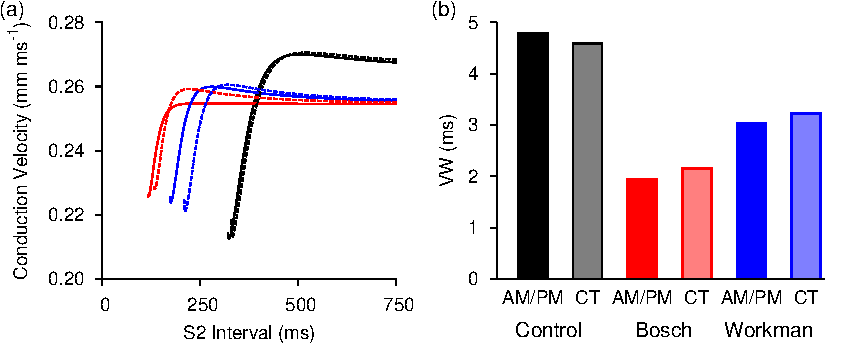
\includegraphics{figures/toolkit/afer/figures/03_CVR}
\caption[AFER CVr curves and VWs]{
\label{fig:toolkit:afer:cvr}
(a) 
CV\emph{r}\ curves for Control (black), Bosch (red) and Workman (blue) tissues.
AM/PM cells are indicated by solid lines, CT cells by dashed.
In all cases CT cells show a higher conduction velocity at long
($>$\ms{600}) S2 intervals, but AM/PM muscles allow faster conduction at lower
S2 intervals.
AF cases show a reduced CV in all instances and support
higher pacing rates via reduced minimal interval.
(b) Vulnerability Window for Control (black), Bosch (red) and Workman (blue).
AM/PM cell types are shown solid, CT are partially shaded.
The VW is reduced for the AF remodelled cases via reduced excitability.
The presence of the remodelling also reverses the difference in VW between cell
types.
}
\end{figure}

Conduction velocity, shown in figure~\ref{fig:toolkit:afer:cvr}(a), was slowed by AF,
reducing the solitary wave velocity from $0.27\,\text{mm}\,\text{ms}^{\text{-1}}$\ in
control to $0.25\,\text{mm}\,\text{ms}^{\text{-1}}$\ in Bosch and
$0.26\,\text{mm}\,\text{ms}^{\text{-1}}$\ in
Workman.
Maximal pacing rate increased from the control value of \unit{187}{bpm} to
\unit{512}{bpm} in Bosch strands and \unit{347}{bpm} in Workman strands of AM or
PM cells.
In CT strands, maximal pacing rates of \unit{183}{bpm}, \unit{451}{bpm}\ and
\unit{287}{bpm}\ were observed for Control, Bosch and Workman cases
respectively.
The heterogeneity of minimal pacing intervals is significantly increased by
AFER, from \unit{4}{bpm}\ to over \unit{50}{bpm}\ in Bosch and Workman strands.

The VW was reduced by AF, figure~\ref{fig:toolkit:afer:cvr}(b).
The control value of \ms{4.8}\ was reduced to \ms{2.0}\ in Bosch and \ms{3.0}\ in Workman for AM and PM cell types.
In CT cells under control conditions, the VW was reduced to \ms{}
The reduction in VW for CT cells was reduced, to \ms{4.6}.
In contrast, the VW increased for AF cases; \ms{2.1}\ and \ms{3.2}\ for Bosch
and Workman cases respectively.


\begin{figure}
\centering
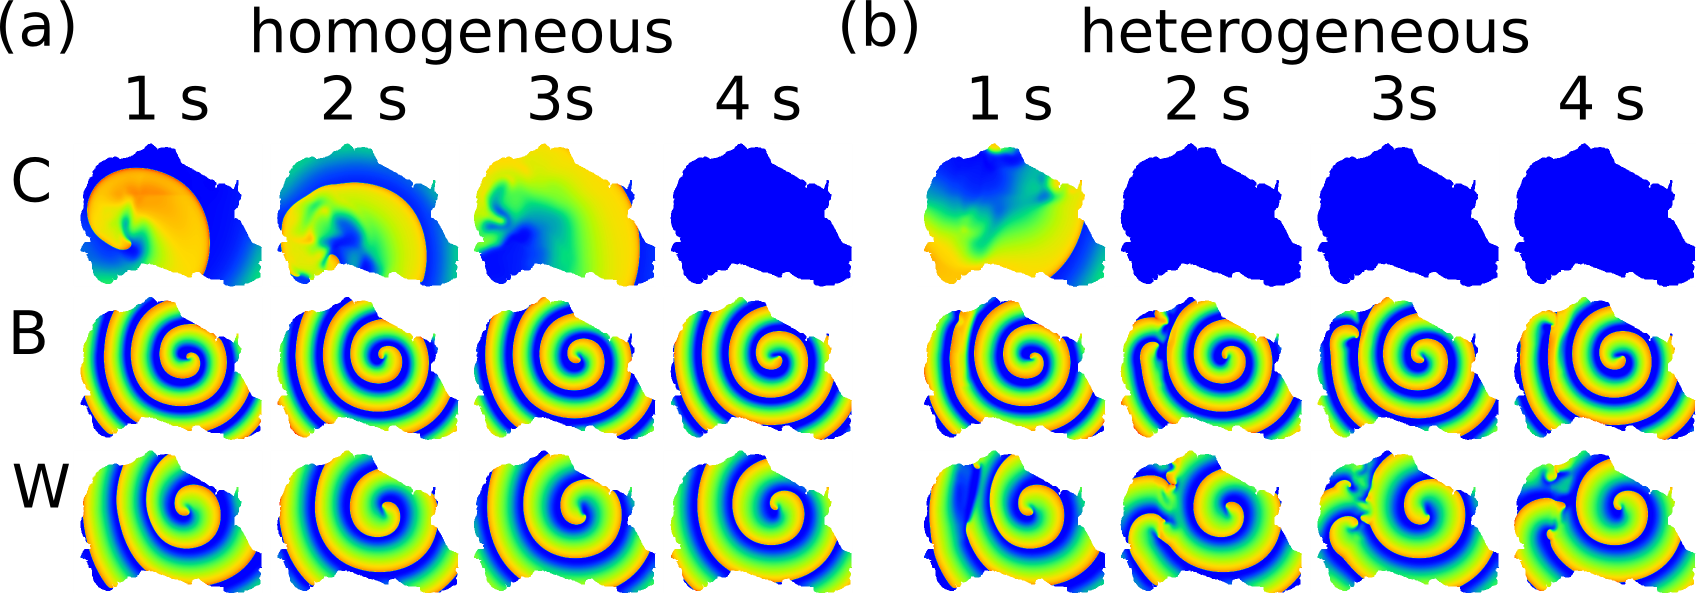
\includegraphics{figures/toolkit/afer/2d_plots}
\caption[AFER 2D re-entry plots]{
\label{fig:toolkit:afer:2d}
Simulation of re-entry in 2D sheets of electrically homogeneous
(a) and electrically heterogeneous (b) sheets.
Colour represents membrane potential from blue (resting) to orange (excited).
Columns show representative frames after initiation of re-entry at t = 0.
Rows C, B, W show data from control, Bosch and Workman cases, respectively.
Re-entry self-terminated under control conditions in both homogeneous (a)(C) and
heterogeneous (a)(C).
Under AF conditions, re-entry becomes a sustained mother rotor in
electrically homogeneous conditions ((a)(B), (a)(W)).
However, under electrically heterogeneous conditions AF causes re-entry to degenerate
into erratic propagations on the borders of the heterogeneity ((b)(B), (b)(W)) }
\end{figure}

Simulations over the 2D geometry examined the lifetime and behaviour of
spiral waves in the presence and absence of electrical heterogeneity.
As can be seen in figure~\ref{fig:toolkit:afer:2d}, panels (a)(C) and (b)(C), re-entrant
activity self-terminated in both homogeneous and heterogeneous cases.
Spiral wave meander over a large region of tissue eventually causes the tip to
leave the tissue.
Self-termination was much more rapid in the electrically heterogeneous case,
taking \unit{1.31}{s}, compared with \unit{3.20}{s} in the homogeneous case.

Conversely, under AF conditions the re-entry persisted after it was
induced for the whole period of the simulation, a lifespan of over \unit{5}{s}.
Under electrically homogeneous conditions, panels (a)(B) and (a)(W) show a
stable mother rotor rotating anti-clockwise in the tissue.
In heterogeneous conditions, as shown in panels (b)(B) and (b)(W), a similar
mother rotor to the homogeneous cases is visible towards the right of each
frame.
On the left of the frames, the rotor breaks up into multiple fibrillatory
wavelets on the border of the heterogeneous regions, forming a complex and
chaotic pattern of excitation.


\subsubsection{Discussion and conclusions}

AFER induces significant changes in the cellular electrophysiology that
appear to affect rate dependent electrical activities.  It helps to
sustain re-entry, providing evidence to substantiate the hypothesis of
`AF begets AF'.

The single cell results show a striking reduction in the \apd\ and
repolarization properties.
AFER abbreviated \apd\ in AM cells by 66~\% in Bosch and 53~\% in Workman.
Other work~\cite{Xie2002,ByungSoo2002,Karma1994,Tusscher2006} has already suggested why flattening of
the ERP and APD restitution curves can be pro-arrhythmogenic.
Our study suggested that reduction is not uniform across all cell types, which
leads to an augmented heterogeneity.

From the 1D results, AFER tissue forms a much better substrate for arrhythmic
activity.
It supports a much higher pacing rate and has a reduced conduction wavelength
(conduction velocity multiplied by \apd), allowing a greater number of
excitation waves to exist in the tissue.
The increase in the heterogeneity of the maximal pacing rates suggests that
remodelled tissues might be more vulnerable to localised regions of conduction
block.
This has been shown to lead to re-entry~\cite{Xie2001a}.

The 2D simulations in the realistic sheet show a marked difference in
re-entrant behavior between homogeneous and heterogeneous simulations.
The homogeneous sheets show self-termination of re-entry in control
tissue, whilst the reduced ERP and conduction wavelength allow the rotor
to remain stable and persist for the duration of the simulation in AFER
condtions as is expected from the flattened restitution
curves~\cite{Xie2002,Karma1994}.
The heterogeneous sheet simulations, show spiral wave
breakup, as observed in real tissue \cite{Kumagai1997}, in both control
and AF simulations, possibly due to elevated plateau potentials and
increased refractory period of the CT cells~\cite{Clayton2005}, combined with
the slower conduction velocity at high pacing rates.
Self-termination is still observed in control simulations and is more rapid than
in homogeneous tissue.

It is still unclear about the pro- or anti-arrhythmogenic effects of
electrical heterogeneity in the human atria.  Self-termination is more
rapid in the heterogeneous tissue for the control case, but despite AFER
increasing the heterogeneity between tissue types, it doesn't lead to
self termination of the re-entry.  In fact, it leads to breakup of the
spiral wave in the region of the heterogeneity, leading to a region of
erratic propagations, as has been seen in experiment~\cite{Kumagai1997}.
Further study, in both 3D geometries and physiological experiments,
would be needed to elucidate the true effects of the heterogeneity.

\section{Discussion and Conclusions}

A cardiac simulation library has been constructed.
This includes implementations of a wide range of experimental protocols used to
classify and quantify the influence on electrophysiology of ion channel changes.
The library of tools was then used in two electrophysiological studies of atrial
tissue.

The cardiac simulation library developed includes experimental protocols used on
lone myocyte models, as well as one- and two-dimensional idealisations of
tissue.
The library of tools is intended to be relatively simple to use and to extend,
although it does require knowledge of programming to use to its full potential
in its present form.
The implementation is intended to be efficient, though without sacrificing
biophysical detail in realistic cell models.
This is accomplished through the use of adaptive stepping methods to track
restitution curves of varying slope, decreasing the gap between data points as
it starts to change more rapidly.
In addition, state saving is performed to reduce the computation involved in
repetitive pre-pacing.
Lookup tables of voltage dependent properties can be employed to further cut
computational time.
The novel use of a very basic computer science algorithm, the binary search, is
used to determine critical values in a number of protocols.
The use of this algorithm allows parameter estimation to great accuracy from
large initial range by successively halving the search space.

Whilst both the binary search and the adaptive step are generally very reliable,
they do on occasion fail dramatically.
This is often caused by incorrect choice of inputs, which don't allow the
algorithm to correctly function, for example, selecting the high and low guesses
for the vulnerable window period too late.
There is unfortunately little that can be done in such cases by the toolkit
itself.
Results might need to be rechecked with a smaller window, centered around the
found time.

The toolkit compares well with many existing frameworks.
COR has many more cells available for use through the CellML repository and
offers an easy way to graph the internal properties of the cell.
Like the library developed here, COR is limited to one OS, which is Microsoft
Windows for COR.
COR has no inbuilt experimental protocols however.
CMISS lacks experimental protocols and is hard to script to use automatically.
It does offer much more sophisticated visualisation than the toolkit here, and
can be used for full 3D simulations too.
CARP offers much more powerful interfaces for cardiac modelling, including 3D
models.
It includes no experimental protocols, although those could probably be
implemented using its API.
Like this toolkit, CARP does not integrate with CellML.

The computational studies reveal the power of the toolkit and the experimental
protocols in assessing the effects of a subtle (\ii{ANION}) and large (AFER)
remodelling of cellular electrophysiological properties.
In the \ii{ANION}\ study, the influence of a novel anion bearing current in the
human atrium was examined.
Despite the small influence of the current on the \apd\ and its time independent
nature, there were significant alterations in the rate dependant and dynamic
behaviours of the cell.
This is due to the voltage at which the current act, and the corresponding
alterations to the time courses of currents which do have time dependent
properties.
The AFER study, by contrast, involved remodelling where many currents were
affected.
In this study, the restitution curves were significantly flattened, leading to
stable spiral waves.
Regional differences in AP profiles, caused by the natural heterogeneity of the
atrium, lead to breakup on the edges of such regions.
